% Options for packages loaded elsewhere
\PassOptionsToPackage{unicode}{hyperref}
\PassOptionsToPackage{hyphens}{url}
%
\documentclass[
]{article}
\usepackage{lmodern}
\usepackage{amssymb,amsmath}
\usepackage{ifxetex,ifluatex}
\ifnum 0\ifxetex 1\fi\ifluatex 1\fi=0 % if pdftex
  \usepackage[T1]{fontenc}
  \usepackage[utf8]{inputenc}
  \usepackage{textcomp} % provide euro and other symbols
\else % if luatex or xetex
  \usepackage{unicode-math}
  \defaultfontfeatures{Scale=MatchLowercase}
  \defaultfontfeatures[\rmfamily]{Ligatures=TeX,Scale=1}
\fi
% Use upquote if available, for straight quotes in verbatim environments
\IfFileExists{upquote.sty}{\usepackage{upquote}}{}
\IfFileExists{microtype.sty}{% use microtype if available
  \usepackage[]{microtype}
  \UseMicrotypeSet[protrusion]{basicmath} % disable protrusion for tt fonts
}{}
\makeatletter
\@ifundefined{KOMAClassName}{% if non-KOMA class
  \IfFileExists{parskip.sty}{%
    \usepackage{parskip}
  }{% else
    \setlength{\parindent}{0pt}
    \setlength{\parskip}{6pt plus 2pt minus 1pt}}
}{% if KOMA class
  \KOMAoptions{parskip=half}}
\makeatother
\usepackage{xcolor}
\IfFileExists{xurl.sty}{\usepackage{xurl}}{} % add URL line breaks if available
\IfFileExists{bookmark.sty}{\usepackage{bookmark}}{\usepackage{hyperref}}
\hypersetup{
  pdftitle={ Cluster Analysis Assignment},
  pdfauthor={Nyasha Mashanda},
  hidelinks,
  pdfcreator={LaTeX via pandoc}}
\urlstyle{same} % disable monospaced font for URLs
\usepackage[margin=1in]{geometry}
\usepackage{color}
\usepackage{fancyvrb}
\newcommand{\VerbBar}{|}
\newcommand{\VERB}{\Verb[commandchars=\\\{\}]}
\DefineVerbatimEnvironment{Highlighting}{Verbatim}{commandchars=\\\{\}}
% Add ',fontsize=\small' for more characters per line
\usepackage{framed}
\definecolor{shadecolor}{RGB}{248,248,248}
\newenvironment{Shaded}{\begin{snugshade}}{\end{snugshade}}
\newcommand{\AlertTok}[1]{\textcolor[rgb]{0.94,0.16,0.16}{#1}}
\newcommand{\AnnotationTok}[1]{\textcolor[rgb]{0.56,0.35,0.01}{\textbf{\textit{#1}}}}
\newcommand{\AttributeTok}[1]{\textcolor[rgb]{0.77,0.63,0.00}{#1}}
\newcommand{\BaseNTok}[1]{\textcolor[rgb]{0.00,0.00,0.81}{#1}}
\newcommand{\BuiltInTok}[1]{#1}
\newcommand{\CharTok}[1]{\textcolor[rgb]{0.31,0.60,0.02}{#1}}
\newcommand{\CommentTok}[1]{\textcolor[rgb]{0.56,0.35,0.01}{\textit{#1}}}
\newcommand{\CommentVarTok}[1]{\textcolor[rgb]{0.56,0.35,0.01}{\textbf{\textit{#1}}}}
\newcommand{\ConstantTok}[1]{\textcolor[rgb]{0.00,0.00,0.00}{#1}}
\newcommand{\ControlFlowTok}[1]{\textcolor[rgb]{0.13,0.29,0.53}{\textbf{#1}}}
\newcommand{\DataTypeTok}[1]{\textcolor[rgb]{0.13,0.29,0.53}{#1}}
\newcommand{\DecValTok}[1]{\textcolor[rgb]{0.00,0.00,0.81}{#1}}
\newcommand{\DocumentationTok}[1]{\textcolor[rgb]{0.56,0.35,0.01}{\textbf{\textit{#1}}}}
\newcommand{\ErrorTok}[1]{\textcolor[rgb]{0.64,0.00,0.00}{\textbf{#1}}}
\newcommand{\ExtensionTok}[1]{#1}
\newcommand{\FloatTok}[1]{\textcolor[rgb]{0.00,0.00,0.81}{#1}}
\newcommand{\FunctionTok}[1]{\textcolor[rgb]{0.00,0.00,0.00}{#1}}
\newcommand{\ImportTok}[1]{#1}
\newcommand{\InformationTok}[1]{\textcolor[rgb]{0.56,0.35,0.01}{\textbf{\textit{#1}}}}
\newcommand{\KeywordTok}[1]{\textcolor[rgb]{0.13,0.29,0.53}{\textbf{#1}}}
\newcommand{\NormalTok}[1]{#1}
\newcommand{\OperatorTok}[1]{\textcolor[rgb]{0.81,0.36,0.00}{\textbf{#1}}}
\newcommand{\OtherTok}[1]{\textcolor[rgb]{0.56,0.35,0.01}{#1}}
\newcommand{\PreprocessorTok}[1]{\textcolor[rgb]{0.56,0.35,0.01}{\textit{#1}}}
\newcommand{\RegionMarkerTok}[1]{#1}
\newcommand{\SpecialCharTok}[1]{\textcolor[rgb]{0.00,0.00,0.00}{#1}}
\newcommand{\SpecialStringTok}[1]{\textcolor[rgb]{0.31,0.60,0.02}{#1}}
\newcommand{\StringTok}[1]{\textcolor[rgb]{0.31,0.60,0.02}{#1}}
\newcommand{\VariableTok}[1]{\textcolor[rgb]{0.00,0.00,0.00}{#1}}
\newcommand{\VerbatimStringTok}[1]{\textcolor[rgb]{0.31,0.60,0.02}{#1}}
\newcommand{\WarningTok}[1]{\textcolor[rgb]{0.56,0.35,0.01}{\textbf{\textit{#1}}}}
\usepackage{longtable,booktabs}
% Correct order of tables after \paragraph or \subparagraph
\usepackage{etoolbox}
\makeatletter
\patchcmd\longtable{\par}{\if@noskipsec\mbox{}\fi\par}{}{}
\makeatother
% Allow footnotes in longtable head/foot
\IfFileExists{footnotehyper.sty}{\usepackage{footnotehyper}}{\usepackage{footnote}}
\makesavenoteenv{longtable}
\usepackage{graphicx,grffile}
\makeatletter
\def\maxwidth{\ifdim\Gin@nat@width>\linewidth\linewidth\else\Gin@nat@width\fi}
\def\maxheight{\ifdim\Gin@nat@height>\textheight\textheight\else\Gin@nat@height\fi}
\makeatother
% Scale images if necessary, so that they will not overflow the page
% margins by default, and it is still possible to overwrite the defaults
% using explicit options in \includegraphics[width, height, ...]{}
\setkeys{Gin}{width=\maxwidth,height=\maxheight,keepaspectratio}
% Set default figure placement to htbp
\makeatletter
\def\fps@figure{htbp}
\makeatother
\setlength{\emergencystretch}{3em} % prevent overfull lines
\providecommand{\tightlist}{%
  \setlength{\itemsep}{0pt}\setlength{\parskip}{0pt}}
\setcounter{secnumdepth}{5}
\usepackage{booktabs}
\usepackage{longtable}
\usepackage{array}
\usepackage{multirow}
\usepackage{wrapfig}
\usepackage{float}
\usepackage{colortbl}
\usepackage{pdflscape}
\usepackage{tabu}
\usepackage{threeparttable}
\usepackage{threeparttablex}
\usepackage[normalem]{ulem}
\usepackage{makecell}
\usepackage{xcolor}

\title{\vspace{3.5in} Cluster Analysis Assignment}
\author{Nyasha Mashanda}
\date{2020-10-17}

\begin{document}
\maketitle

{
\setcounter{tocdepth}{2}
\tableofcontents
}
\newpage 
\tableofcontents 
\listoffigures
\listoftables
\newpage

\begin{Shaded}
\begin{Highlighting}[]
\KeywordTok{library}\NormalTok{(kableExtra)}
\end{Highlighting}
\end{Shaded}

\begin{verbatim}
## 
## Attaching package: 'kableExtra'
\end{verbatim}

\begin{verbatim}
## The following object is masked from 'package:dplyr':
## 
##     group_rows
\end{verbatim}

\begin{Shaded}
\begin{Highlighting}[]
\CommentTok{# Display this on the first page to see what and from where each variable was collected.}
\NormalTok{owid_covid_codebook <-}\StringTok{ }\KeywordTok{read_csv}\NormalTok{(}\StringTok{"owid-covid-codebook.csv"}\NormalTok{)}
\end{Highlighting}
\end{Shaded}

\begin{verbatim}
## Parsed with column specification:
## cols(
##   Variable = col_character(),
##   Description = col_character()
## )
\end{verbatim}

\begin{Shaded}
\begin{Highlighting}[]
\NormalTok{knitr}\OperatorTok{::}\KeywordTok{kable}\NormalTok{(owid_covid_codebook, }\DataTypeTok{digits =} \DecValTok{5}\NormalTok{, }\DataTypeTok{caption =} \StringTok{"Acronyms"}\NormalTok{) }\OperatorTok
\StringTok{  }\KeywordTok{kable_styling}\NormalTok{(}\DataTypeTok{full_width =}\NormalTok{ F, }\DataTypeTok{font_size =} \DecValTok{7}\NormalTok{) }\OperatorTok
\StringTok{  }\KeywordTok{column_spec}\NormalTok{(}\DecValTok{1}\NormalTok{, }\DataTypeTok{border_left =}\NormalTok{ T) }\OperatorTok
\StringTok{  }\KeywordTok{column_spec}\NormalTok{(}\DecValTok{2}\NormalTok{, }\DataTypeTok{border_right =}\NormalTok{ T)}
\end{Highlighting}
\end{Shaded}

\begin{table}

\caption{\label{tab:acronyms-tab}Acronyms}
\centering
\fontsize{7}{9}\selectfont
\begin{tabular}[t]{|>{}l|>{}l|}
\hline
Variable & Description\\
\hline
iso\_code & ISO 3166-1 alpha-3 – three-letter country codes\\
\hline
continent & Continent of the geographical location\\
\hline
location & Geographical location\\
\hline
date & Date of observation\\
\hline
total\_cases & Total confirmed cases of COVID-19\\
\hline
new\_cases & New confirmed cases of COVID-19\\
\hline
new\_cases\_smoothed & New confirmed cases of COVID-19 (7-day smoothed)\\
\hline
total\_deaths & Total deaths attributed to COVID-19\\
\hline
new\_deaths & New deaths attributed to COVID-19\\
\hline
new\_deaths\_smoothed & New deaths attributed to COVID-19 (7-day smoothed)\\
\hline
total\_cases\_per\_million & Total confirmed cases of COVID-19 per 1,000,000 people\\
\hline
new\_cases\_per\_million & New confirmed cases of COVID-19 per 1,000,000 people\\
\hline
new\_cases\_smoothed\_per\_million & New confirmed cases of COVID-19 (7-day smoothed) per 1,000,000 people\\
\hline
total\_deaths\_per\_million & Total deaths attributed to COVID-19 per 1,000,000 people\\
\hline
new\_deaths\_per\_million & New deaths attributed to COVID-19 per 1,000,000 people\\
\hline
new\_deaths\_smoothed\_per\_million & New deaths attributed to COVID-19 (7-day smoothed) per 1,000,000 people\\
\hline
population\_density & Number of people divided by land area, measured in square kilometers\\
\hline
median\_age & Median age of the population, UN projection for 2020\\
\hline
aged\_65\_older & Share of the population that is 65 years and older, most recent year available\\
\hline
aged\_70\_older & Share of the population that is 70 years and older in 2015\\
\hline
gdp\_per\_capita & Gross domestic product at purchasing power parity (constant 2011 international dollars)\\
\hline
extreme\_poverty & Share of the population living in extreme poverty, most recent year available since 2010\\
\hline
cardiovasc\_death\_rate & Death rate from cardiovascular disease in 2017 (annual number of deaths per 100,000 people)\\
\hline
diabetes\_prevalence & Diabetes prevalence (\% of population aged 20 to 79) in 2017\\
\hline
female\_smokers & Share of women who smoke, most recent year available\\
\hline
male\_smokers & Share of men who smoke, most recent year available\\
\hline
handwashing\_facilities & Share of the population with basic handwashing facilities on premises\\
\hline
hospital\_beds\_per\_thousand & Hospital beds per 1,000 people, most recent year available since 2010\\
\hline
life\_expectancy & Life expectancy at birth in 2019\\
\hline
\end{tabular}
\end{table}

\begin{Shaded}
\begin{Highlighting}[]
\CommentTok{#View(owid_covid_codebook)}
\end{Highlighting}
\end{Shaded}

\newpage
\abstract

The novel COVID-19 corona virus is still not well understood and there are many open questions related to patterns in its spread. The goal of this assignment is to discover if there are any regional patterns that exist using cluster analysis.

The assignment uses COVD-19 pandemic data collected from the Our World In Data site (European Center for Disease Prevention and Control 2020). The data contains 29 indicators related to the
COVID-19 cases for 208 countries. The data set is updated daily from when the pandemic started. For this assignment, a subset of the
data will be used; this subset consists of all the information on the pandemic on the 02 of September
2020.

There are three kinds of clustering methods that will be explored in this analysis: hierarchical, partitioning and density based methods. In order to determine any regional patterns, the number of clusters will be limited to 6, resembling the six regions that are: Africa, Asia, Europe, North America, Oceania and South America.

\pagebreak

\hypertarget{what-about-standardising-the-data}{%
\section{What about standardising the data????}\label{what-about-standardising-the-data}}

\hypertarget{exploratory-data-analysis}{%
\section{Exploratory Data Analysis}\label{exploratory-data-analysis}}

\begin{Shaded}
\begin{Highlighting}[]
\CommentTok{# Reading the data}
\NormalTok{df1 <-}\StringTok{ }\KeywordTok{read_excel}\NormalTok{(}\StringTok{"owid-covid-data.xlsx"}\NormalTok{, }\DataTypeTok{sheet =} \StringTok{"Data"}\NormalTok{)}

\CommentTok{# Check if data has been imported correctly}
\KeywordTok{head}\NormalTok{(df1) }
\end{Highlighting}
\end{Shaded}

\begin{verbatim}
## # A tibble: 6 x 30
##   location iso_code continent date  total_cases new_cases new_cases_smoot~
##   <chr>    <chr>    <chr>     <chr>       <dbl>     <dbl>            <dbl>
## 1 Algeria  DZA      Africa    2020~       44833       339           372.  
## 2 Angola   AGO      Africa    2020~        2654        30            53   
## 3 Benin    BEN      Africa    2020~        2145         0             4.29
## 4 Botswana BWA      Africa    2020~        1733         9            24.4 
## 5 Burkina~ BFA      Africa    2020~        1375         5             3.29
## 6 Burundi  BDI      Africa    2020~         445         0             2.14
## # ... with 23 more variables: total_deaths <dbl>, new_deaths <dbl>,
## #   new_deaths_smoothed <dbl>, total_cases_per_million <dbl>,
## #   new_cases_per_million <dbl>, new_cases_smoothed_per_million <dbl>,
## #   total_deaths_per_million <dbl>, new_deaths_per_million <dbl>,
## #   new_deaths_smoothed_per_million <dbl>, population <dbl>,
## #   population_density <dbl>, median_age <dbl>, aged_65_older <dbl>,
## #   aged_70_older <dbl>, gdp_per_capita <dbl>, extreme_poverty <dbl>,
## #   cardiovasc_death_rate <dbl>, diabetes_prevalence <dbl>,
## #   female_smokers <dbl>, male_smokers <dbl>, handwashing_facilities <dbl>,
## #   hospital_beds_per_thousand <dbl>, life_expectancy <dbl>
\end{verbatim}

\begin{Shaded}
\begin{Highlighting}[]
\KeywordTok{tail}\NormalTok{(df1)}
\end{Highlighting}
\end{Shaded}

\begin{verbatim}
## # A tibble: 6 x 30
##   location iso_code continent date  total_cases new_cases new_cases_smoot~
##   <chr>    <chr>    <chr>     <chr>       <dbl>     <dbl>            <dbl>
## 1 Guyana   GUY      South Am~ 2020~        1373        67             44.7
## 2 Paraguay PRY      South Am~ 2020~       18338       676            587. 
## 3 Peru     PER      South Am~ 2020~      657129      5092           7107. 
## 4 Suriname SUR      South Am~ 2020~        4089        55             55.9
## 5 Uruguay  URY      South Am~ 2020~        1611        16             10.7
## 6 Venezue~ VEN      South Am~ 2020~       47756      1888            943. 
## # ... with 23 more variables: total_deaths <dbl>, new_deaths <dbl>,
## #   new_deaths_smoothed <dbl>, total_cases_per_million <dbl>,
## #   new_cases_per_million <dbl>, new_cases_smoothed_per_million <dbl>,
## #   total_deaths_per_million <dbl>, new_deaths_per_million <dbl>,
## #   new_deaths_smoothed_per_million <dbl>, population <dbl>,
## #   population_density <dbl>, median_age <dbl>, aged_65_older <dbl>,
## #   aged_70_older <dbl>, gdp_per_capita <dbl>, extreme_poverty <dbl>,
## #   cardiovasc_death_rate <dbl>, diabetes_prevalence <dbl>,
## #   female_smokers <dbl>, male_smokers <dbl>, handwashing_facilities <dbl>,
## #   hospital_beds_per_thousand <dbl>, life_expectancy <dbl>
\end{verbatim}

\begin{Shaded}
\begin{Highlighting}[]
\CommentTok{# Look at the structure of the data}
\KeywordTok{str}\NormalTok{(df1)}
\end{Highlighting}
\end{Shaded}

\begin{verbatim}
## tibble [208 x 30] (S3: tbl_df/tbl/data.frame)
##  $ location                       : chr [1:208] "Algeria" "Angola" "Benin" "Botswana" ...
##  $ iso_code                       : chr [1:208] "DZA" "AGO" "BEN" "BWA" ...
##  $ continent                      : chr [1:208] "Africa" "Africa" "Africa" "Africa" ...
##  $ date                           : chr [1:208] "2020-09-02" "2020-09-02" "2020-09-02" "2020-09-02" ...
##  $ total_cases                    : num [1:208] 44833 2654 2145 1733 1375 ...
##  $ new_cases                      : num [1:208] 339 30 0 9 5 0 267 86 0 4 ...
##  $ new_cases_smoothed             : num [1:208] 372.14 53 4.29 24.43 3.29 ...
##  $ total_deaths                   : num [1:208] 1518 108 40 6 55 ...
##  $ new_deaths                     : num [1:208] 8 1 0 0 0 0 3 0 0 0 ...
##  $ new_deaths_smoothed            : num [1:208] 8.857 0.857 0.143 0.429 0 ...
##  $ total_cases_per_million        : num [1:208] 1022.4 80.8 176.9 736.9 65.8 ...
##  $ new_cases_per_million          : num [1:208] 7.731 0.913 0 3.827 0.239 ...
##  $ new_cases_smoothed_per_million : num [1:208] 8.487 1.613 0.354 10.388 0.157 ...
##  $ total_deaths_per_million       : num [1:208] 34.62 3.29 3.3 2.55 2.63 ...
##  $ new_deaths_per_million         : num [1:208] 0.182 0.03 0 0 0 0 0.113 0 0 0 ...
##  $ new_deaths_smoothed_per_million: num [1:208] 0.202 0.026 0.012 0.182 0 0 0.022 0.771 0.03 0 ...
##  $ population                     : num [1:208] 43851043 32866268 12123198 2351625 20903278 ...
##  $ population_density             : num [1:208] 17.35 23.89 99.11 4.04 70.15 ...
##  $ median_age                     : num [1:208] 29.1 16.8 18.8 25.8 17.6 17.5 18.8 25.7 18.3 16.7 ...
##  $ aged_65_older                  : num [1:208] 6.21 2.4 3.24 3.94 2.41 ...
##  $ aged_70_older                  : num [1:208] 3.86 1.36 1.94 2.24 1.36 ...
##  $ gdp_per_capita                 : num [1:208] 13914 5819 2064 15807 1703 ...
##  $ extreme_poverty                : num [1:208] 0.5 NA 49.6 NA 43.7 71.7 23.8 NA NA 38.4 ...
##  $ cardiovasc_death_rate          : num [1:208] 278 276 236 237 269 ...
##  $ diabetes_prevalence            : num [1:208] 6.73 3.94 0.99 4.81 2.42 6.05 7.2 2.42 6.1 6.1 ...
##  $ female_smokers                 : num [1:208] 0.7 NA 0.6 5.7 1.6 NA NA 2.1 NA NA ...
##  $ male_smokers                   : num [1:208] 30.4 NA 12.3 34.4 23.9 NA NA 16.5 NA NA ...
##  $ handwashing_facilities         : num [1:208] 83.7 26.7 11 NA 11.9 ...
##  $ hospital_beds_per_thousand     : num [1:208] 1.9 NA 0.5 1.8 0.4 0.8 1.3 2.1 1 NA ...
##  $ life_expectancy                : num [1:208] 76.9 61.1 61.8 69.6 61.6 ...
\end{verbatim}

The data was exported to a dataframe from an excel file ``owid-covid-data.xlsx''. The first step is to check if the data has been imported correctly using the head() and tail() functions. This was confirmed by running the code. The next step included checking the structure of the dataframe and also the variables in the data (See variables in Table \ref{tab:acronyms-tab}). Location, iso\_code, continent and date were found to be in character format while the rest of the variables are numerical. This is fine expcept for the date which should be in a date format. However, since this column has only one date, the column will not be used for ana;ysis and will be removed from the dataframe.

The next step is to visualize the distribution of the variables and this will be done using box and whisker plots.

\hypertarget{distribution}{%
\subsection{Distribution}\label{distribution}}

\hypertarget{cluster-analysis}{%
\section{Cluster Analysis}\label{cluster-analysis}}

\hypertarget{k-means}{%
\subsection{K-means}\label{k-means}}

\hypertarget{k-mediods}{%
\subsection{K-mediods}\label{k-mediods}}

\hypertarget{clara}{%
\subsection{Clara}\label{clara}}

\hypertarget{dbscan}{%
\subsection{DBSCAN}\label{dbscan}}

\hypertarget{dimension-reduction}{%
\section{Dimension Reduction}\label{dimension-reduction}}

\hypertarget{results}{%
\subsection{Results}\label{results}}

The data shows that handwashing\_facilties, extreme poverty, male smokers and female smokers are among the columns with the highest percentages of missing data.

\begin{Shaded}
\begin{Highlighting}[]
\CommentTok{# Plot box and whisker for all variables}

\NormalTok{df1 }\OperatorTok
\StringTok{  }\KeywordTok{keep}\NormalTok{(is.numeric) }\OperatorTok
\StringTok{  }\KeywordTok{select}\NormalTok{(}\KeywordTok{c}\NormalTok{(}\DecValTok{1}\OperatorTok{:}\DecValTok{8}\NormalTok{)) }\OperatorTok
\StringTok{  }\KeywordTok{gather}\NormalTok{() }\OperatorTok\StringTok{ }
\StringTok{  }\KeywordTok{ggplot}\NormalTok{(}\KeywordTok{aes}\NormalTok{(value)) }\OperatorTok{+}
\StringTok{    }\KeywordTok{facet_wrap}\NormalTok{(}\OperatorTok{~}\StringTok{ }\NormalTok{key, }\DataTypeTok{scales =} \StringTok{"free"}\NormalTok{) }\OperatorTok{+}
\StringTok{    }\KeywordTok{geom_boxplot}\NormalTok{(}
      \CommentTok{# custom boxes}
        \DataTypeTok{color=}\StringTok{"blue"}\NormalTok{,}
        \DataTypeTok{fill=}\StringTok{"blue"}\NormalTok{,}
        \DataTypeTok{alpha=}\FloatTok{0.2}\NormalTok{,}
        
        \CommentTok{# Notch?}
        \DataTypeTok{notch=}\OtherTok{TRUE}\NormalTok{,}
        \DataTypeTok{notchwidth =} \FloatTok{0.8}\NormalTok{,}
        
        \CommentTok{# custom outliers}
        \DataTypeTok{outlier.colour=}\StringTok{"black"}\NormalTok{,}
        \DataTypeTok{outlier.fill=}\StringTok{"black"}\NormalTok{,}
        \DataTypeTok{outlier.size=}\DecValTok{2}
\NormalTok{    )}
\end{Highlighting}
\end{Shaded}

\begin{verbatim}
## notch went outside hinges. Try setting notch=FALSE.
## notch went outside hinges. Try setting notch=FALSE.
\end{verbatim}

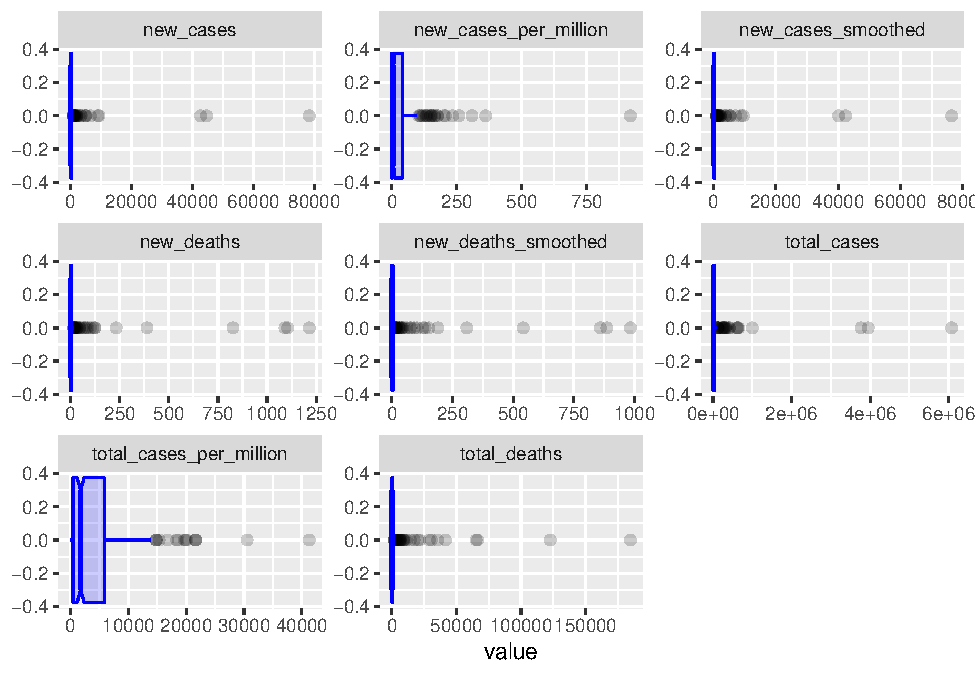
\includegraphics{Assignment1_files/figure-latex/unnamed-chunk-2-1.pdf}

The first seven figures shpw that most of the data is concerntrated very close to less than a thousand except for total\_cases\_per\_million which is more spread and between 0 and 5000. All the variables contain numerous outliers and this shows that we might need a clustering method that is robust and not affected by outliers.

\begin{Shaded}
\begin{Highlighting}[]
\NormalTok{df1 }\OperatorTok
\StringTok{  }\KeywordTok{keep}\NormalTok{(is.numeric) }\OperatorTok
\StringTok{  }\KeywordTok{select}\NormalTok{(}\KeywordTok{c}\NormalTok{(}\DecValTok{9}\OperatorTok{:}\DecValTok{16}\NormalTok{)) }\OperatorTok
\StringTok{  }\KeywordTok{gather}\NormalTok{() }\OperatorTok\StringTok{ }
\StringTok{  }\KeywordTok{ggplot}\NormalTok{(}\KeywordTok{aes}\NormalTok{(value)) }\OperatorTok{+}
\StringTok{    }\KeywordTok{facet_wrap}\NormalTok{(}\OperatorTok{~}\StringTok{ }\NormalTok{key, }\DataTypeTok{scales =} \StringTok{"free"}\NormalTok{) }\OperatorTok{+}
\StringTok{    }\KeywordTok{geom_boxplot}\NormalTok{(}
            \CommentTok{# custom boxes}
        \DataTypeTok{color=}\StringTok{"blue"}\NormalTok{,}
        \DataTypeTok{fill=}\StringTok{"blue"}\NormalTok{,}
        \DataTypeTok{alpha=}\FloatTok{0.2}\NormalTok{,}
        
        \CommentTok{# Notch?}
        \DataTypeTok{notch=}\OtherTok{TRUE}\NormalTok{,}
        \DataTypeTok{notchwidth =} \FloatTok{0.8}\NormalTok{,}
        
        \CommentTok{# custom outliers}
        \DataTypeTok{outlier.colour=}\StringTok{"black"}\NormalTok{,}
        \DataTypeTok{outlier.fill=}\StringTok{"black"}\NormalTok{,}
        \DataTypeTok{outlier.size=}\DecValTok{2}
\NormalTok{    )}
\end{Highlighting}
\end{Shaded}

\begin{verbatim}
## Warning: Removed 62 rows containing non-finite values (stat_boxplot).
\end{verbatim}

\begin{verbatim}
## notch went outside hinges. Try setting notch=FALSE.
## notch went outside hinges. Try setting notch=FALSE.
\end{verbatim}

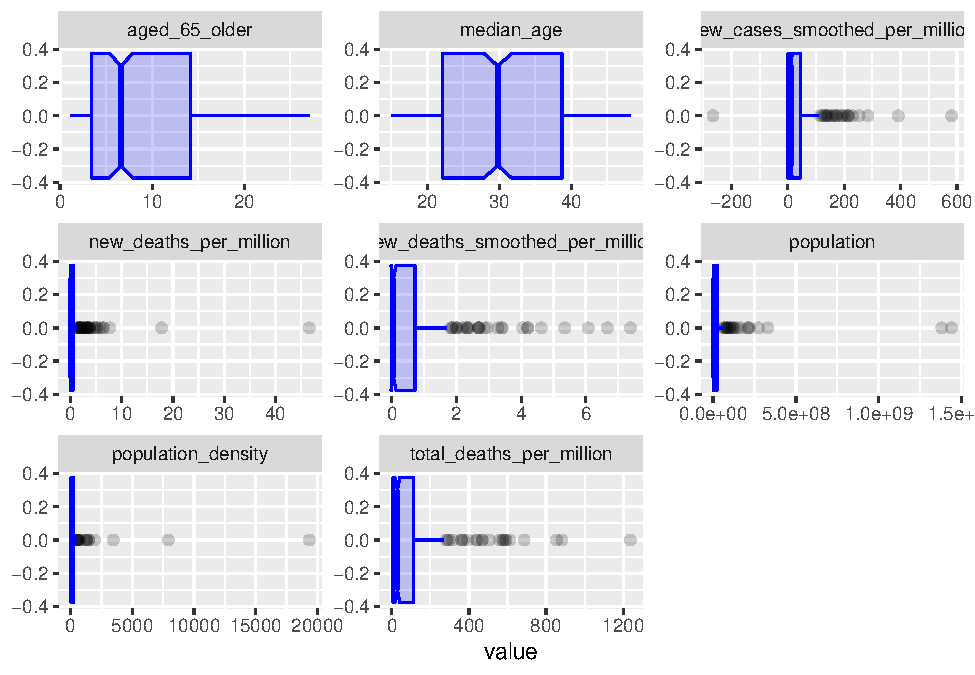
\includegraphics{Assignment1_files/figure-latex/unnamed-chunk-3-1.pdf}
Almost half of the variables
Median\_age and aged\_65\_older values are much more spread. The numbers seem resasonable given that a smaller percentage of the population is age above 65 and usually the median age of most countries is expected to be below 50 given that there usually more young people than older people in country. Countries like Japan and Italy seem to have the highest percentage of older people with a median age of 48.2 and 47.9. The Niger and Uganda have the youngest population with a median age of 16.1 and 15.4. In genral European countries seems to have an older society while Africa countries have a much younger population.

Monaco and Singapore have the highstest population densities while China has the highest population. As a result these countries stand out as outliers with regards to population variables.

New Deaths per million are hightest in north and south america.

New cases smoothed per million show a negative number(outlier). This is most likely a entry error and the values will be replaced with a regional average.

\begin{Shaded}
\begin{Highlighting}[]
\NormalTok{df1 }\OperatorTok
\StringTok{  }\KeywordTok{keep}\NormalTok{(is.numeric) }\OperatorTok
\StringTok{  }\KeywordTok{select}\NormalTok{(}\KeywordTok{c}\NormalTok{(}\DecValTok{17}\OperatorTok{:}\DecValTok{25}\NormalTok{)) }\OperatorTok
\StringTok{  }\KeywordTok{gather}\NormalTok{() }\OperatorTok\StringTok{ }
\StringTok{  }\KeywordTok{ggplot}\NormalTok{(}\KeywordTok{aes}\NormalTok{(value)) }\OperatorTok{+}
\StringTok{    }\KeywordTok{facet_wrap}\NormalTok{(}\OperatorTok{~}\StringTok{ }\NormalTok{key, }\DataTypeTok{scales =} \StringTok{"free"}\NormalTok{) }\OperatorTok{+}
\StringTok{    }\KeywordTok{geom_boxplot}\NormalTok{(}
            \CommentTok{# custom boxes}
        \DataTypeTok{color=}\StringTok{"blue"}\NormalTok{,}
        \DataTypeTok{fill=}\StringTok{"blue"}\NormalTok{,}
        \DataTypeTok{alpha=}\FloatTok{0.2}\NormalTok{,}
        
        \CommentTok{# Notch?}
        \DataTypeTok{notch=}\OtherTok{TRUE}\NormalTok{,}
        \DataTypeTok{notchwidth =} \FloatTok{0.8}\NormalTok{,}
        
        \CommentTok{# custom outliers}
        \DataTypeTok{outlier.colour=}\StringTok{"black"}\NormalTok{,}
        \DataTypeTok{outlier.fill=}\StringTok{"black"}\NormalTok{,}
        \DataTypeTok{outlier.size=}\DecValTok{2}
\NormalTok{    )}
\end{Highlighting}
\end{Shaded}

\begin{verbatim}
## Warning: Removed 483 rows containing non-finite values (stat_boxplot).
\end{verbatim}

\begin{verbatim}
## notch went outside hinges. Try setting notch=FALSE.
\end{verbatim}

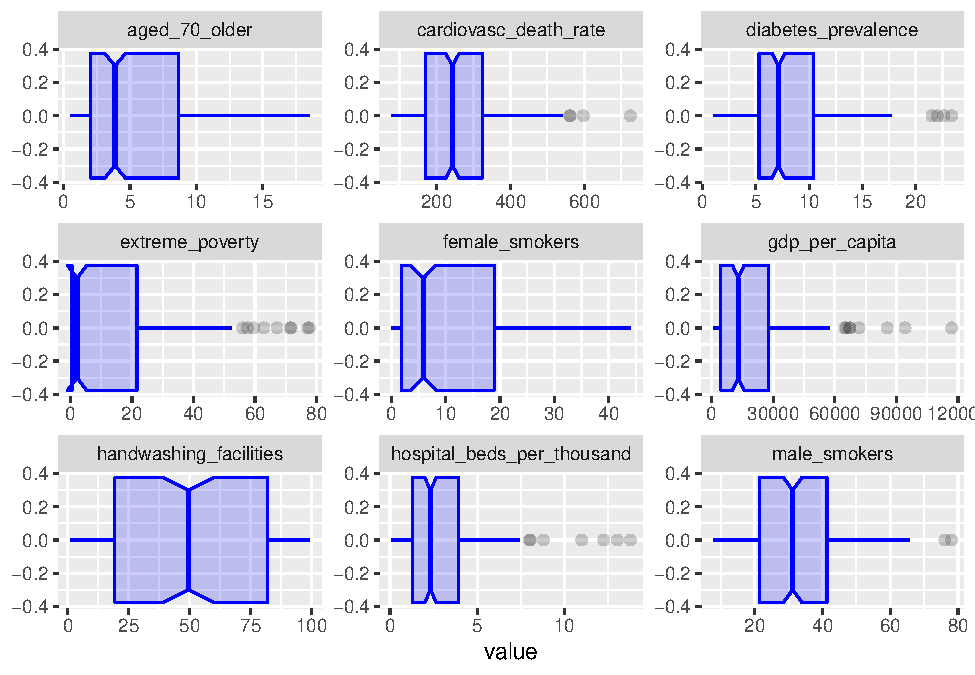
\includegraphics{Assignment1_files/figure-latex/unnamed-chunk-4-1.pdf}

The observations for these variables look more spread with less outliers. The variables also suggest that there are generally more male smokers than female smokers. Futhermore, the data show that it is mostly european countries that are wealthy or less poor. The numbers seem to be in the expected ranges.

\hypertarget{missing-values}{%
\subsection{Missing values}\label{missing-values}}

Running a summary on the dataframe shows that there are various columns with missing data.

\begin{Shaded}
\begin{Highlighting}[]
\NormalTok{missing_data_visual <-}\StringTok{ }\KeywordTok{vis_miss}\NormalTok{(df1, }\DataTypeTok{sort_miss =}\NormalTok{ T) }\CommentTok{# Visualise to see rows/columns with missing data}
\CommentTok{#missing_data_visual}

\NormalTok{aggr_plot <-}\StringTok{ }\NormalTok{VIM}\OperatorTok{::}\KeywordTok{aggr}\NormalTok{(df1, }\DataTypeTok{col=}\KeywordTok{c}\NormalTok{(}\StringTok{'navyblue'}\NormalTok{,}\StringTok{'red'}\NormalTok{), }\DataTypeTok{numbers=}\OtherTok{TRUE}\NormalTok{, }\DataTypeTok{sortVars=}\OtherTok{TRUE}\NormalTok{, }\DataTypeTok{labels=}\KeywordTok{names}\NormalTok{(df1), }\DataTypeTok{cex.axis=}\NormalTok{.}\DecValTok{5}\NormalTok{, }\DataTypeTok{gap=}\DecValTok{3}\NormalTok{, }\DataTypeTok{ylab=}\KeywordTok{c}\NormalTok{(}\StringTok{"Histogram of missing data"}\NormalTok{,}\StringTok{"Pattern"}\NormalTok{), }\DataTypeTok{plot =}\NormalTok{ F)}
\KeywordTok{plot}\NormalTok{(aggr_plot, }\DataTypeTok{cex.axis=}\NormalTok{.}\DecValTok{5}\NormalTok{, }\DataTypeTok{gap=}\DecValTok{3}\NormalTok{, }\DataTypeTok{ylab=}\KeywordTok{c}\NormalTok{(}\StringTok{"Histogram of missing data"}\NormalTok{,}\StringTok{"Pattern"}\NormalTok{))}
\end{Highlighting}
\end{Shaded}

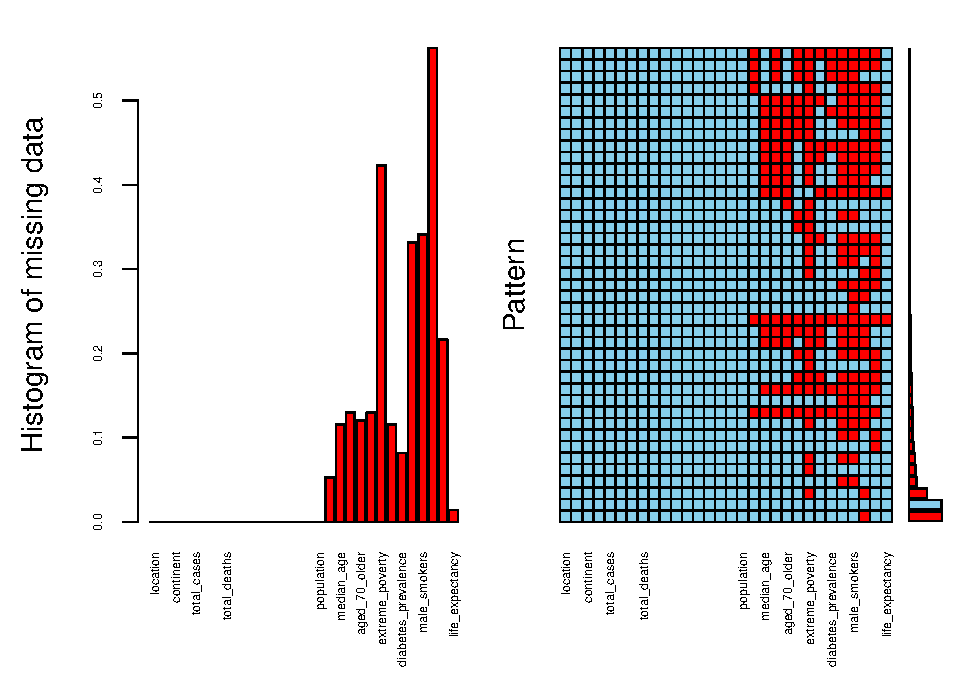
\includegraphics{Assignment1_files/figure-latex/missing_data_tab-1.pdf}

\begin{Shaded}
\begin{Highlighting}[]
\CommentTok{# Creating table}
\NormalTok{missing_data_table =}\StringTok{ }\NormalTok{aggr_plot}\OperatorTok{$}\NormalTok{missings }\OperatorTok
\StringTok{  }\KeywordTok{filter}\NormalTok{(Count }\OperatorTok{>}\StringTok{ }\DecValTok{0}\NormalTok{) }\OperatorTok
\StringTok{  }\KeywordTok{arrange}\NormalTok{(}\KeywordTok{desc}\NormalTok{(Count)) }\OperatorTok
\StringTok{  }\KeywordTok{mutate}\NormalTok{(}\DataTypeTok{Percentage =}\NormalTok{ Count}\OperatorTok{/}\DecValTok{208}\NormalTok{)}

\NormalTok{knitr}\OperatorTok{::}\KeywordTok{kable}\NormalTok{(missing_data_table, }\DataTypeTok{digits =} \DecValTok{5}\NormalTok{, }\DataTypeTok{caption =} \StringTok{"Missing data visualisation"}\NormalTok{) }\OperatorTok
\StringTok{  }\KeywordTok{kable_styling}\NormalTok{(}\DataTypeTok{full_width =}\NormalTok{ F, }\DataTypeTok{font_size =} \DecValTok{7}\NormalTok{) }\OperatorTok
\StringTok{  }\KeywordTok{column_spec}\NormalTok{(}\DecValTok{1}\NormalTok{, }\DataTypeTok{border_left =}\NormalTok{ T) }\OperatorTok
\StringTok{  }\KeywordTok{column_spec}\NormalTok{(}\DecValTok{3}\NormalTok{, }\DataTypeTok{border_right =}\NormalTok{ T)}
\end{Highlighting}
\end{Shaded}

\textbackslash begin\{table\}

\textbackslash caption\{(\#tab:missing\_data\_tab)Missing data visualisation\}
\centering
\fontsize{7}{9}\selectfont

\begin{tabular}[t]{|>{}l|r|>{}r|}
\hline
Variable & Count & Percentage\\
\hline
handwashing\_facilities & 117 & 0.56250\\
\hline
extreme\_poverty & 88 & 0.42308\\
\hline
male\_smokers & 71 & 0.34135\\
\hline
female\_smokers & 69 & 0.33173\\
\hline
hospital\_beds\_per\_thousand & 45 & 0.21635\\
\hline
aged\_65\_older & 27 & 0.12981\\
\hline
gdp\_per\_capita & 27 & 0.12981\\
\hline
aged\_70\_older & 25 & 0.12019\\
\hline
median\_age & 24 & 0.11538\\
\hline
cardiovasc\_death\_rate & 24 & 0.11538\\
\hline
diabetes\_prevalence & 17 & 0.08173\\
\hline
population\_density & 11 & 0.05288\\
\hline
life\_expectancy & 3 & 0.01442\\
\hline
\end{tabular}

\textbackslash end\{table\}

As show in Table @ref(missing\_data\_tab), a number of variables have a very high number of missing values including handwashing\_facilities, extreme\_poverty, male smokers and female smokers. It is generally not ggod working with data or columns that have a high percentage of missing data. Therefore various methods of imputing the missing data will be observed in the next section.

\hypertarget{imputation-by-data-scrapping}{%
\subsection{Imputation by data scrapping}\label{imputation-by-data-scrapping}}

There are various sources that were used to collect the data including the European Center for Disease Prevention and Control. However some of the data can be found on wikipedia. Although the data will not exactly be the same but the values will be very similar.

Over 78\% of rows have missing data therefore simply omitting the rows with missing will lead to a loss a huge size of important data.

Population density missing values were imputed using the data from wikipedia ({\textbf{???}} Density) \url{https://en.wikipedia.org/wiki/List_of_countries_and_dependencies_by_population_density}

It is important to indicate that the data was given in 2019 but given that population densities change very slowly, this is better than replacing with an average/median.

Median age missing values will be imputed using the data found from the following wikipedia site: \url{https://en.wikipedia.org/wiki/List_of_countries_by_median_age}

Median ages data was added using data from the 2019 data \url{https://www.cia.gov/library/publications/the-world-factbook/fields/343rank.html}

Only data for Syria was found.

Median age above 75 years old was ignored

Searching the source of the data maps to a site: \url{https://github.com/owid/covid-19-data/blob/master/public/data/owid-covid-codebook.csv} which says the gdp\_per\_capita Gross domestic product at purchasing power parity (constant 2011 international dollars), most recent year available. Given that the most recent data from the world bank (\url{https://databank.worldbank.org/source/jobs/Series/NY.GDP.PCAP.PP.KD\#}) which matches this data is for the year 2016, the data was used for imputing the data. Note the data is not available

Extreme poverty is a population with an income of less than \$1.90 a day. From the data the Share of the population living in extreme poverty, most recent year available since 2010. The data from the following site \url{https://en.wikipedia.org/wiki/List_of_countries_by_percentage_of_population_living_in_poverty} the data is very similar to that available without missing values, therefore it will be better to use the data for imputing.

Most countries with 0 percent were having missing values

This was skipped due to insufficient data to fill in the missing values.

female and male smokers info not enough
handwashing facilities skipped because data is not enough.
hospital bed per thousand informatiion was found to be too old for example Chad which had data for 2005. Given that there are many years between the time the data was collected and this year the data was ignored.

From the world bank data on life expectancy ( \url{https://data.worldbank.org/indicator/SP.DYN.LE00.IN} ), the life expectancy of Guernsey, Jersey and Kosovo are 82.6, 80.6, 71.95 years respectively.

\begin{center}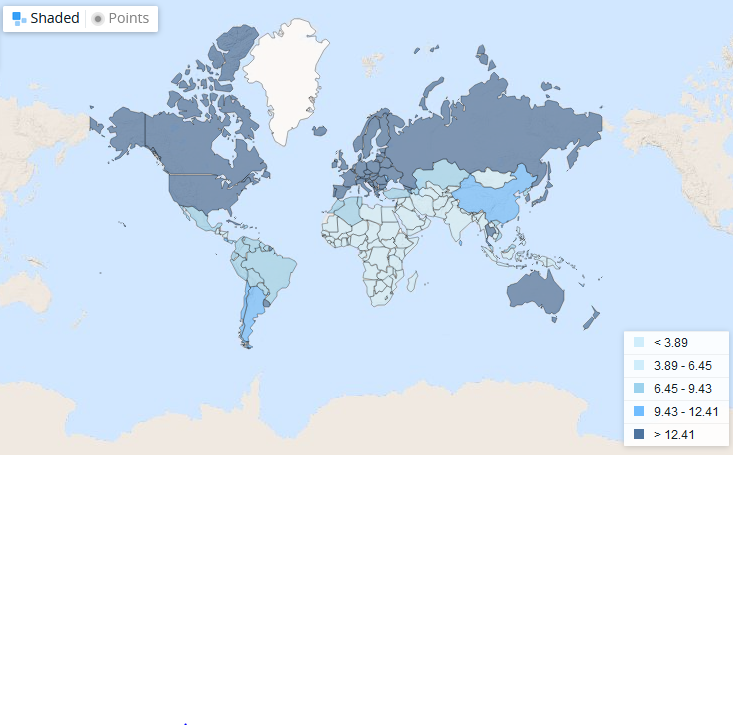
\includegraphics[width=1\linewidth,height=1\textheight]{Capture} \end{center}

The results show that handwashing\_facilites is missing 56.25\% of the values followed by extreme\_poverty missing 42.3\% of the values. In total, 78.4\% of the samples have missing values.

The histograms also suggest that there is a negative value in new\_cases\_smoothed\_per\_million.

Upon further investigation, Luxembourg seems to have negative values for new\_cases\_smoothed and new\_cases\_smoothed\_per\_million. This is probably because the new\_cases\_smoothed\_per\_million is derived from new\_cases\_smoothed.

The mice package allows multivariate imputation by chained equations

MICE assumes that the missing data are Missing at Random (MAR), which means that the propensity for a data point to be missing is not related to the missing data but is related to some of the observed data.
\url{https://www.theanalysisfactor.com/mar-and-mcar-missing-data/}

Therefore it is important to determine which columns have data points that may be missing at random. The imputation process is not a one size fits all method.

There is also the Amelia package which also makes an assumption that the missing data is random in nature (MSR)

Hmisc is a multiple purpose package useful for data analysis, high -- level graphics, imputing missing values, advanced table making, model fitting \& diagnostics (linear regression, logistic regression \& cox regression) etc. Hmisc assumes linearity in the variables being predicted.

mi (Multiple imputation with diagnostics) package provides several features for dealing with missing values. Like other packages, it also builds multiple imputation models to approximate missing values. And, uses predictive mean matching method like the mice package.

The following variables need need impiutation using some of the methods.

\hypertarget{female_smokers-and-male_smokers-cardiovasc_death_rate-and-diabetes-prevalence-are-macr-variables-therefore-the-mice-package-will-be-used-on-this-data.}{%
\subsection{female\_smokers and male\_smokers, cardiovasc\_death\_rate and diabetes prevalence are MACR variables therefore the MICE package will be used on this data.}\label{female_smokers-and-male_smokers-cardiovasc_death_rate-and-diabetes-prevalence-are-macr-variables-therefore-the-mice-package-will-be-used-on-this-data.}}

various packages will be used for imputation and the one that yields the best result will be chosen.

This will be support for dimension reduction.

It is not enough to try out one package for imputing data therefore try out more!
The question is if any one value of the observation is missing, will it affect the missingness of a specific variable.

The percentage of population aged\_65\_older looks to have regional patterns therefore it is justified to use regional medians/averages for imputation. Since aged\_70\_older can is closely related to aged\_65\_older it is decided to use the same method.

The randomizing, re-running, averaging and final run is a very good advice.

\begin{Shaded}
\begin{Highlighting}[]
\CommentTok{# Hierarchical clustering}
\CommentTok{# Compute pairwise distance matrices}
\NormalTok{dist.out <-}\StringTok{ }\KeywordTok{dist}\NormalTok{(data.out,}
                 \DataTypeTok{method =} \StringTok{"euclidean"}\NormalTok{)}
\CommentTok{# Hierarchical clustering results}
\NormalTok{hc <-}\StringTok{ }\KeywordTok{hclust}\NormalTok{(dist.out,}
             \DataTypeTok{method =} \StringTok{"complete"}\NormalTok{)}
\CommentTok{# Visualization of hclust}
\KeywordTok{plot}\NormalTok{(hc, }\DataTypeTok{labels =}\NormalTok{ F,}\OperatorTok{-}\DecValTok{1}\NormalTok{)}
\end{Highlighting}
\end{Shaded}

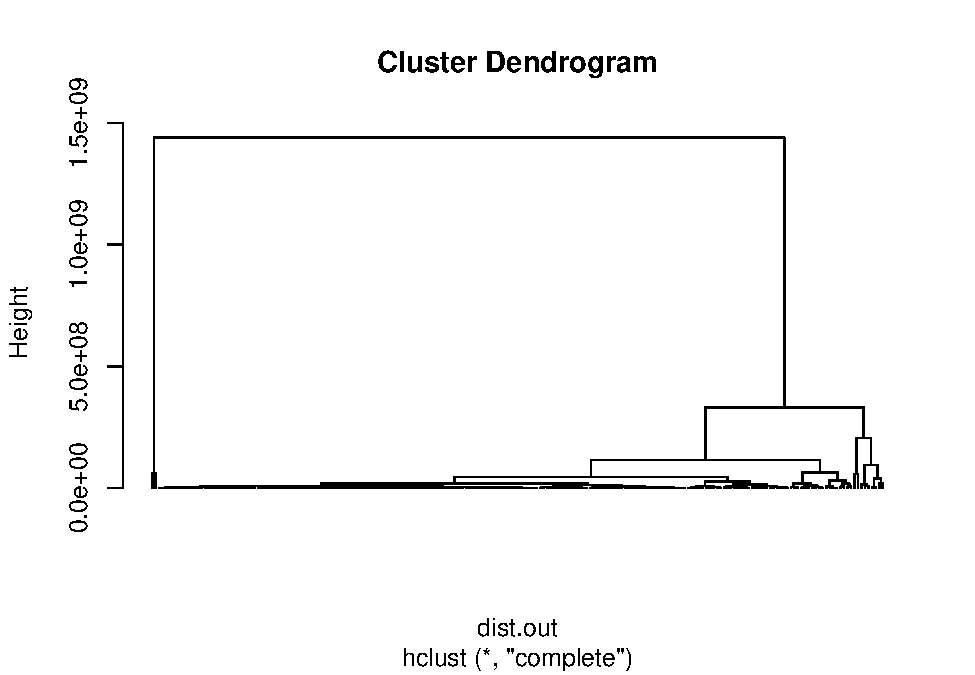
\includegraphics{Assignment1_files/figure-latex/unnamed-chunk-26-1.pdf}

\begin{Shaded}
\begin{Highlighting}[]
\KeywordTok{plot}\NormalTok{(}\KeywordTok{silhouette}\NormalTok{(}\KeywordTok{cutree}\NormalTok{(hc,}\DecValTok{6}\NormalTok{),dist.out))}
\end{Highlighting}
\end{Shaded}

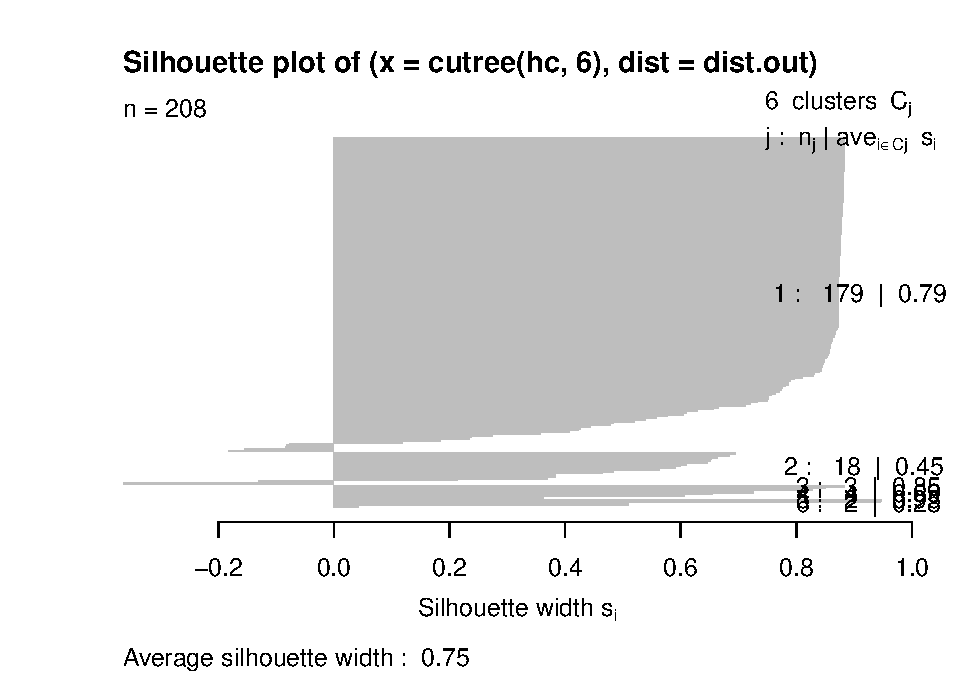
\includegraphics{Assignment1_files/figure-latex/unnamed-chunk-26-2.pdf}

\begin{Shaded}
\begin{Highlighting}[]
\NormalTok{hc <-}\StringTok{ }\KeywordTok{hclust}\NormalTok{(dist.out,}
             \DataTypeTok{method =} \StringTok{"complete"}\NormalTok{)}
\CommentTok{# Visualization of hclust}
\KeywordTok{plot}\NormalTok{(hc, }\DataTypeTok{labels =}\NormalTok{ F,}\OperatorTok{-}\DecValTok{1}\NormalTok{)}
\end{Highlighting}
\end{Shaded}

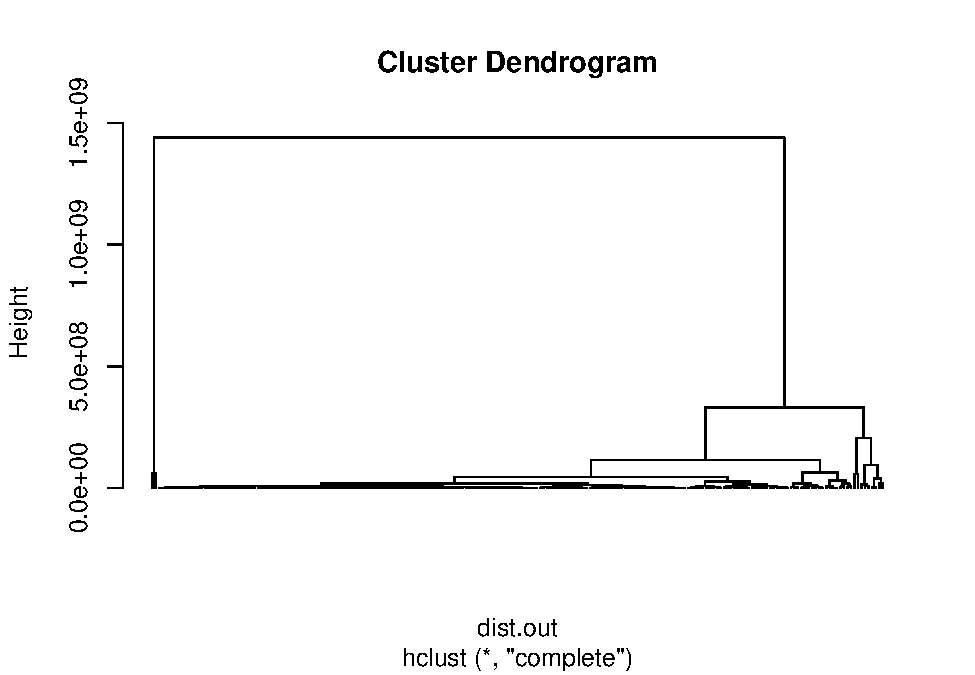
\includegraphics{Assignment1_files/figure-latex/unnamed-chunk-26-3.pdf}

\begin{Shaded}
\begin{Highlighting}[]
\KeywordTok{plot}\NormalTok{(}\KeywordTok{silhouette}\NormalTok{(}\KeywordTok{cutree}\NormalTok{(hc,}\DecValTok{6}\NormalTok{),dist.out))}
\end{Highlighting}
\end{Shaded}

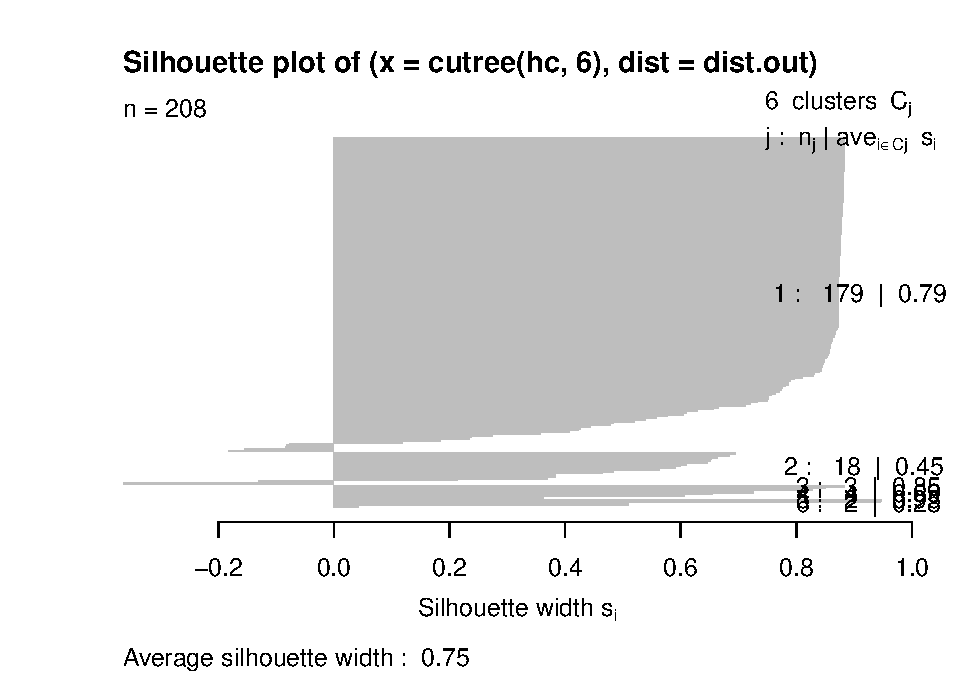
\includegraphics{Assignment1_files/figure-latex/unnamed-chunk-26-4.pdf}

\begin{Shaded}
\begin{Highlighting}[]
\NormalTok{hc <-}\StringTok{ }\KeywordTok{hclust}\NormalTok{(dist.out,}
             \DataTypeTok{method =} \StringTok{"single"}\NormalTok{)}
\CommentTok{# Visualization of hclust}
\KeywordTok{plot}\NormalTok{(hc, }\DataTypeTok{labels =}\NormalTok{ F,}\OperatorTok{-}\DecValTok{1}\NormalTok{)}
\end{Highlighting}
\end{Shaded}

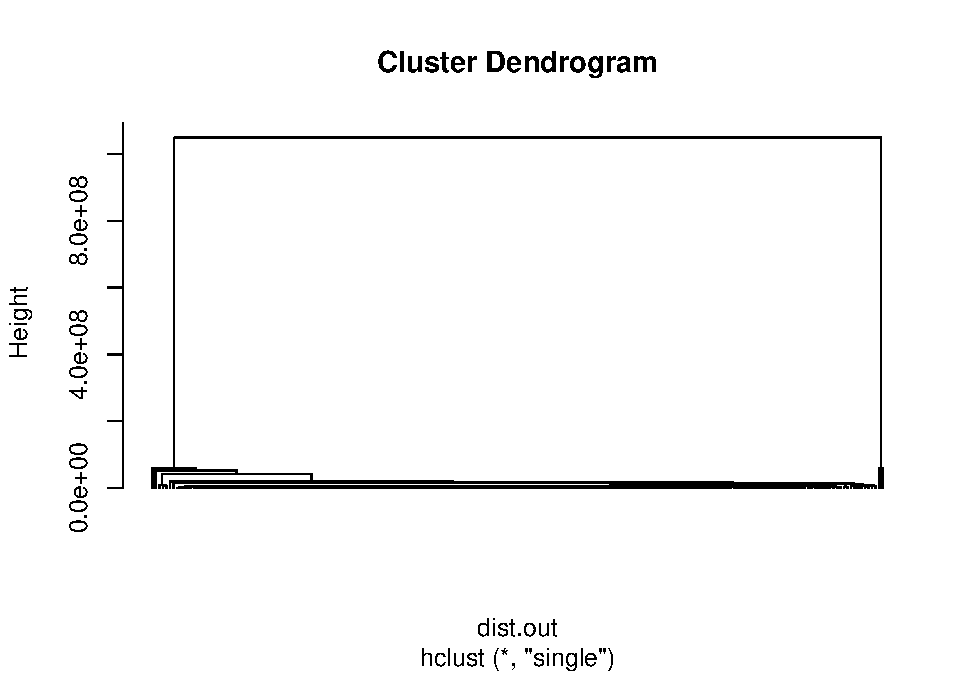
\includegraphics{Assignment1_files/figure-latex/unnamed-chunk-26-5.pdf}

\begin{Shaded}
\begin{Highlighting}[]
\KeywordTok{plot}\NormalTok{(}\KeywordTok{silhouette}\NormalTok{(}\KeywordTok{cutree}\NormalTok{(hc,}\DecValTok{6}\NormalTok{),dist.out))}
\end{Highlighting}
\end{Shaded}

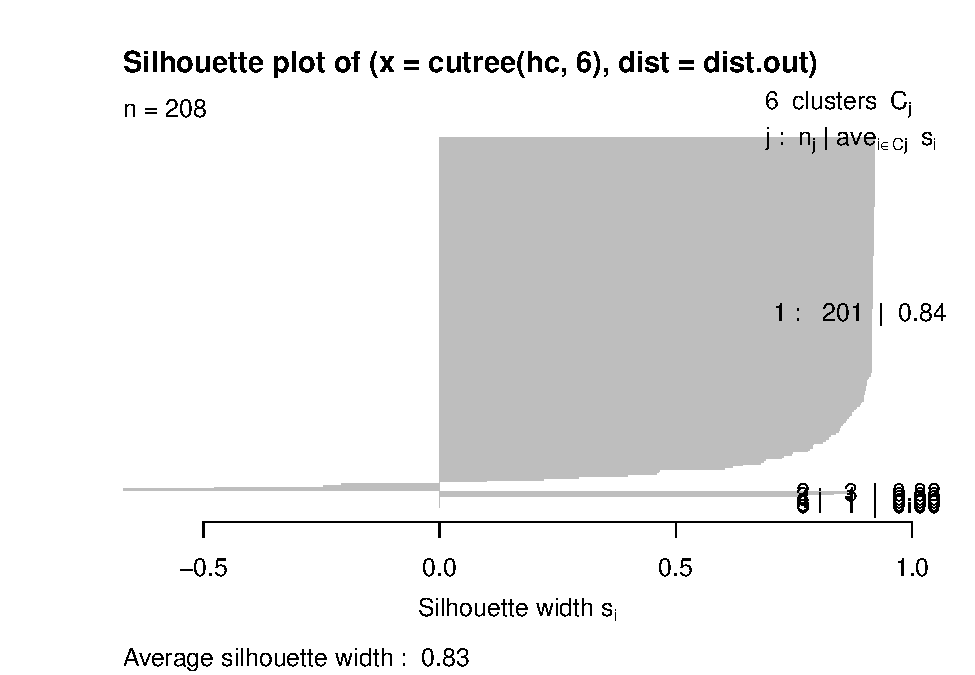
\includegraphics{Assignment1_files/figure-latex/unnamed-chunk-26-6.pdf}

\begin{Shaded}
\begin{Highlighting}[]
\NormalTok{hc <-}\StringTok{ }\KeywordTok{hclust}\NormalTok{(dist.out,}
             \DataTypeTok{method =} \StringTok{"average"}\NormalTok{)}
\CommentTok{# Visualization of hclust}
\KeywordTok{plot}\NormalTok{(hc, }\DataTypeTok{labels =}\NormalTok{ F,}\OperatorTok{-}\DecValTok{1}\NormalTok{)}
\end{Highlighting}
\end{Shaded}

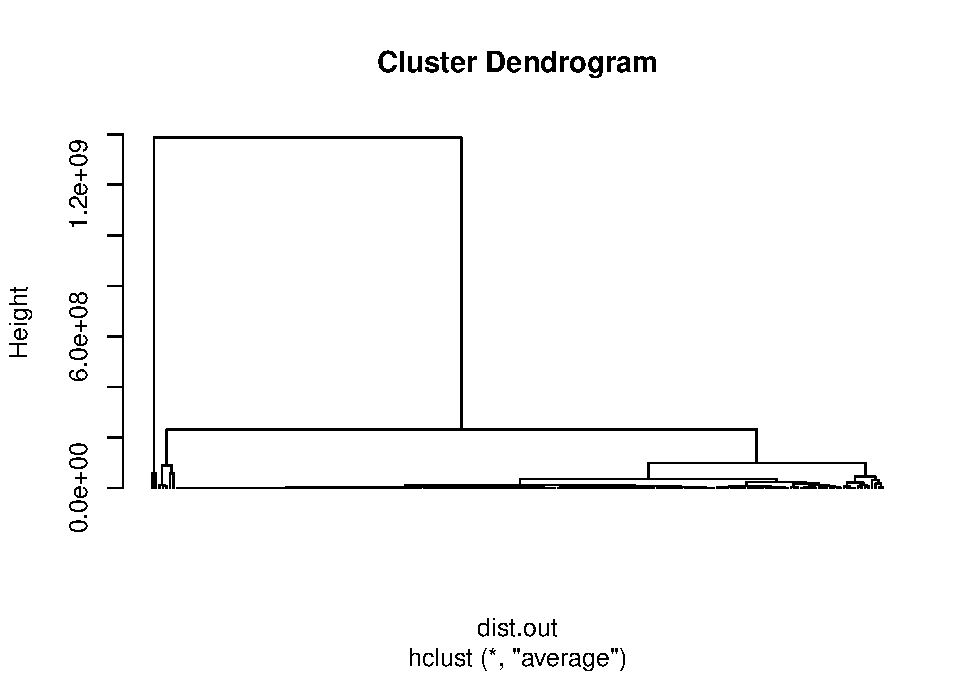
\includegraphics{Assignment1_files/figure-latex/unnamed-chunk-26-7.pdf}

\begin{Shaded}
\begin{Highlighting}[]
\KeywordTok{plot}\NormalTok{(}\KeywordTok{silhouette}\NormalTok{(}\KeywordTok{cutree}\NormalTok{(hc,}\DecValTok{6}\NormalTok{),dist.out))}
\end{Highlighting}
\end{Shaded}

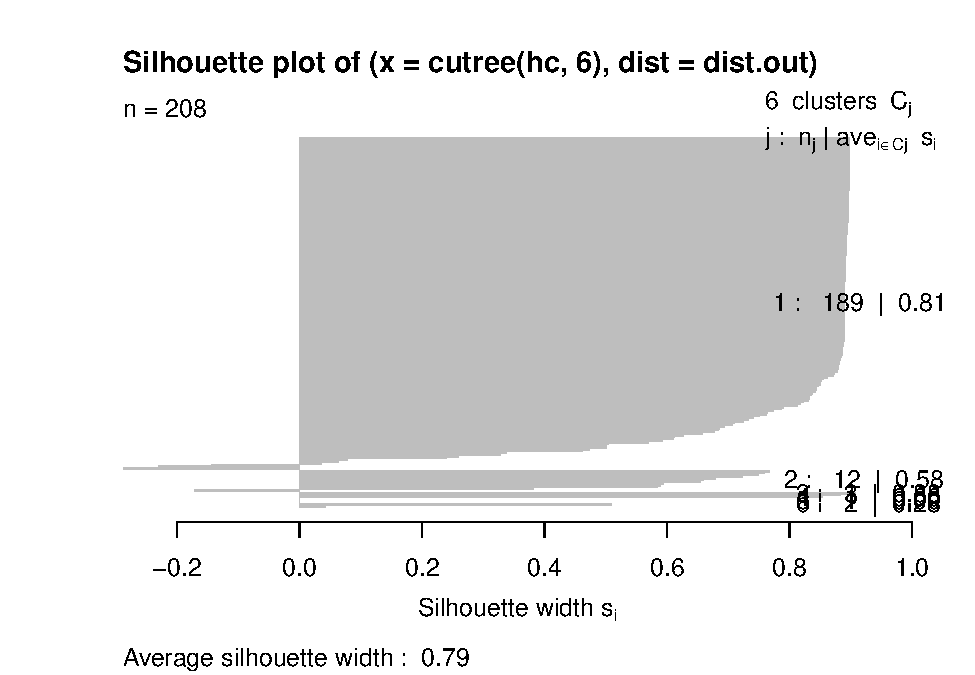
\includegraphics{Assignment1_files/figure-latex/unnamed-chunk-26-8.pdf}

\begin{Shaded}
\begin{Highlighting}[]
\NormalTok{hc <-}\StringTok{ }\KeywordTok{hclust}\NormalTok{(dist.out,}
             \DataTypeTok{method =} \StringTok{"median"}\NormalTok{)}
\CommentTok{# Visualization of hclust}
\KeywordTok{plot}\NormalTok{(hc, }\DataTypeTok{labels =}\NormalTok{ F,}\OperatorTok{-}\DecValTok{1}\NormalTok{)}
\end{Highlighting}
\end{Shaded}

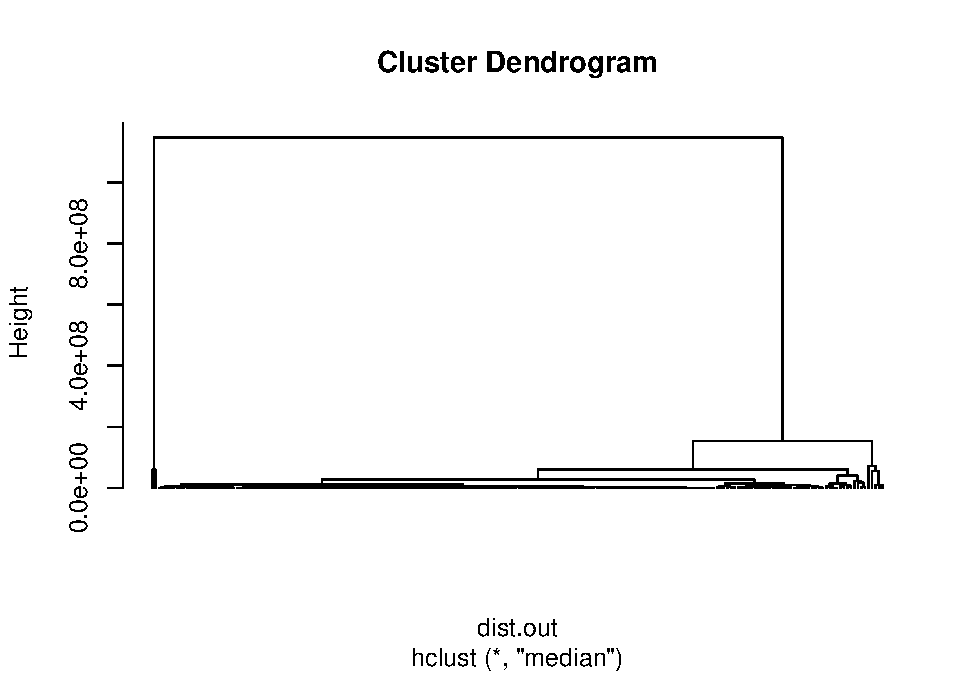
\includegraphics{Assignment1_files/figure-latex/unnamed-chunk-26-9.pdf}

\begin{Shaded}
\begin{Highlighting}[]
\KeywordTok{plot}\NormalTok{(}\KeywordTok{silhouette}\NormalTok{(}\KeywordTok{cutree}\NormalTok{(hc,}\DecValTok{6}\NormalTok{),dist.out))}
\end{Highlighting}
\end{Shaded}

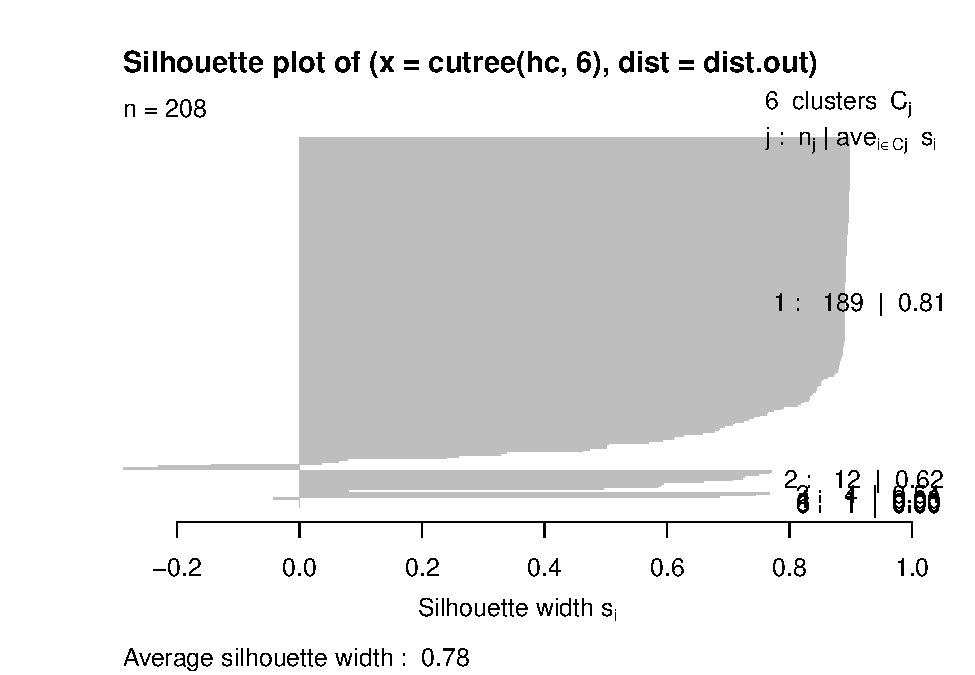
\includegraphics{Assignment1_files/figure-latex/unnamed-chunk-26-10.pdf}

\begin{Shaded}
\begin{Highlighting}[]
\NormalTok{hc <-}\StringTok{ }\KeywordTok{hclust}\NormalTok{(dist.out,}
             \DataTypeTok{method =} \StringTok{"centroid"}\NormalTok{)}
\CommentTok{# Visualization of hclust}
\KeywordTok{plot}\NormalTok{(hc, }\DataTypeTok{labels =}\NormalTok{ F,}\OperatorTok{-}\DecValTok{1}\NormalTok{)}
\end{Highlighting}
\end{Shaded}

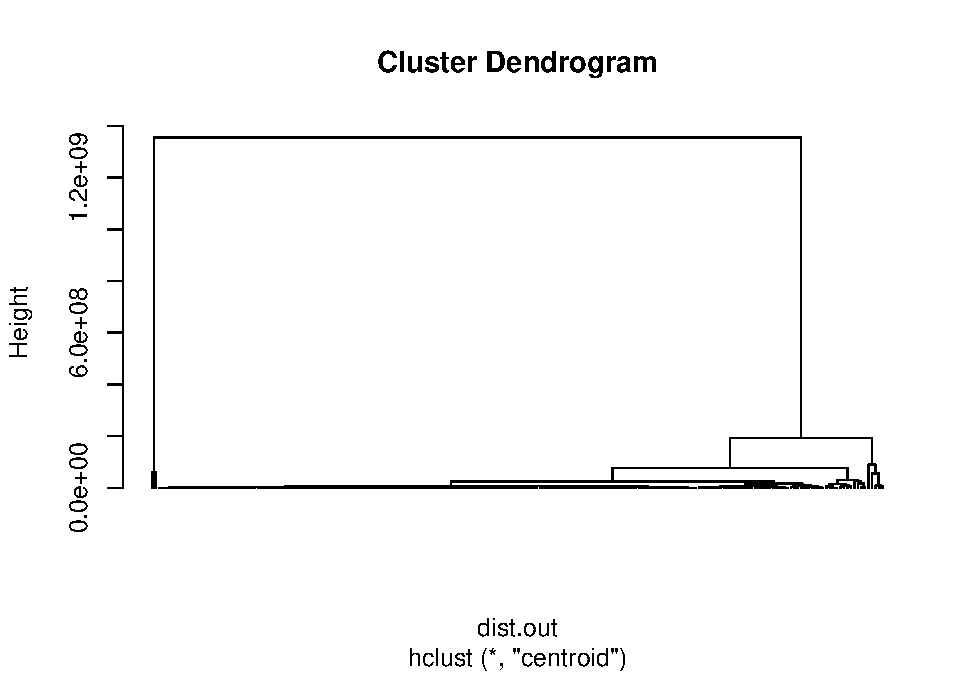
\includegraphics{Assignment1_files/figure-latex/unnamed-chunk-26-11.pdf}

\begin{Shaded}
\begin{Highlighting}[]
\KeywordTok{plot}\NormalTok{(}\KeywordTok{silhouette}\NormalTok{(}\KeywordTok{cutree}\NormalTok{(hc,}\DecValTok{6}\NormalTok{),dist.out))}
\end{Highlighting}
\end{Shaded}

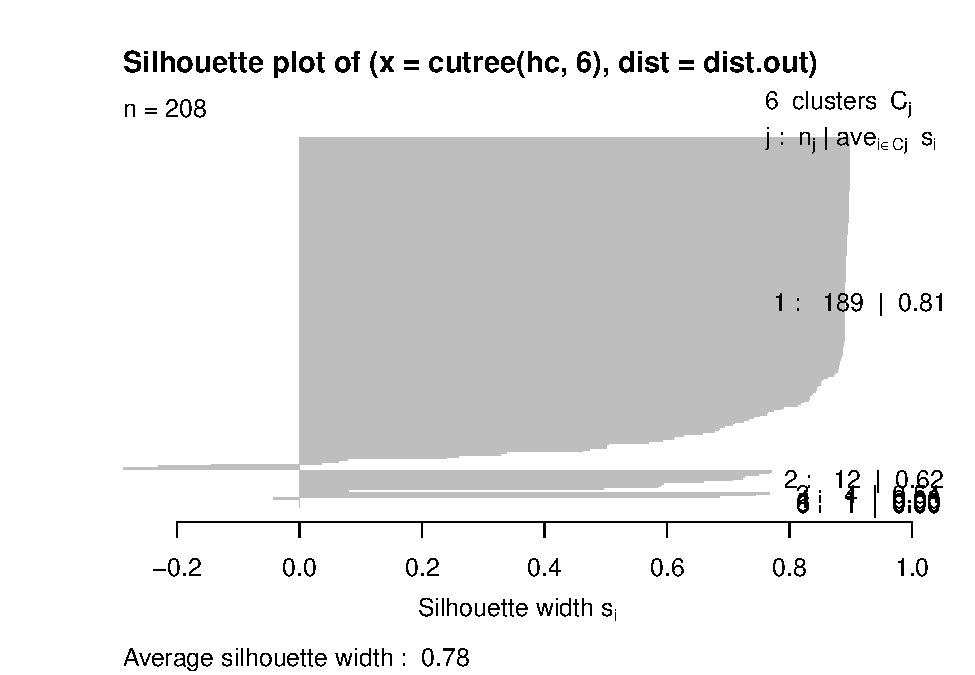
\includegraphics{Assignment1_files/figure-latex/unnamed-chunk-26-12.pdf}

\begin{Shaded}
\begin{Highlighting}[]
\CommentTok{# # }
\CommentTok{# rect.hclust(hc, k = 6, border = 2:3)}
\CommentTok{# }
\CommentTok{# hcd <- as.dendrogram(hc)}
\CommentTok{# # Define nodePar}
\CommentTok{# nodePar <- list(lab.cex = 0.6,}
\CommentTok{#                 pch = c(20, 19),}
\CommentTok{#                 cex = 0.7,}
\CommentTok{#                 col = c("green","yellow"))}
\CommentTok{# plot(hcd,}
\CommentTok{#      xlab = "Height",}
\CommentTok{#      nodePar = nodePar,}
\CommentTok{#      main = "Cluster dendrogram",}
\CommentTok{#      edgePar = list(col = c("red","blue"), lwd = 2:1),}
\CommentTok{#      horiz = TRUE)}
\end{Highlighting}
\end{Shaded}

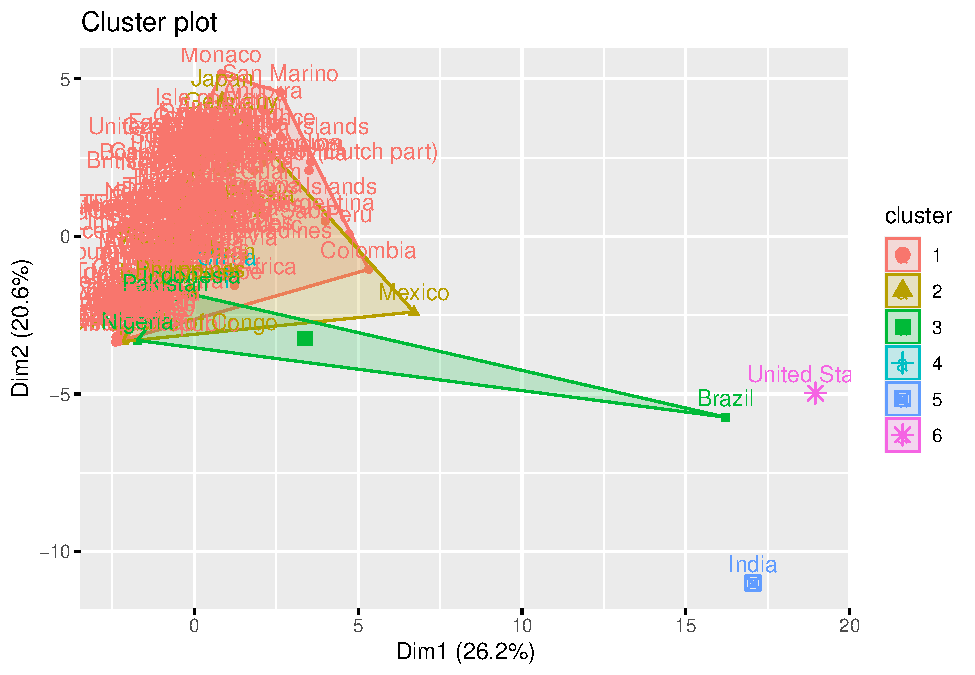
\includegraphics{Assignment1_files/figure-latex/unnamed-chunk-27-1.pdf}

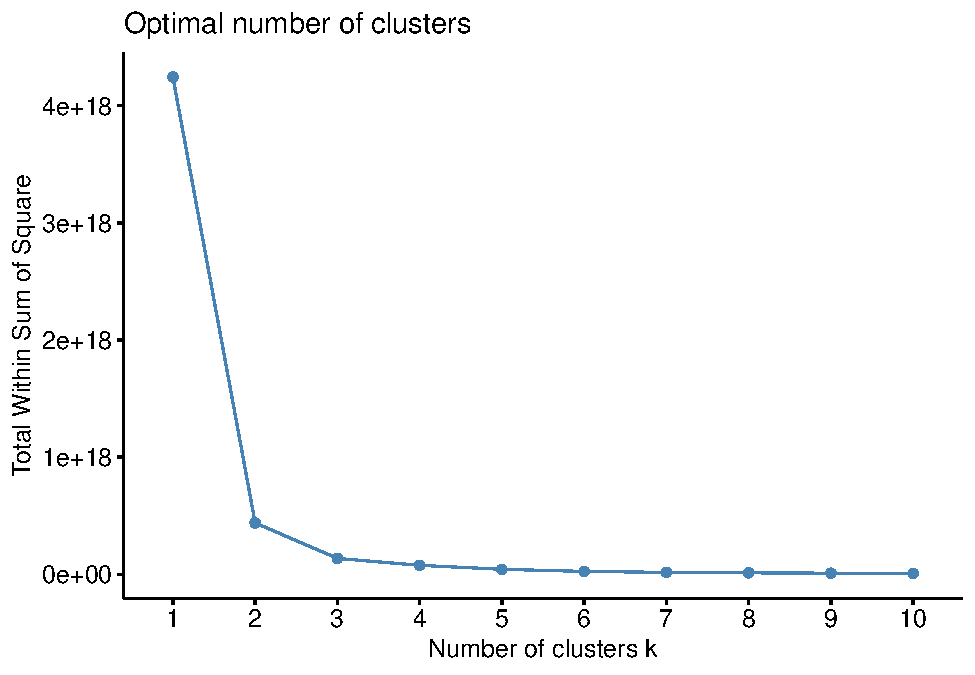
\includegraphics{Assignment1_files/figure-latex/unnamed-chunk-28-1.pdf}

The dataset is very small and this results in Clara performing worse than PAM.

The randomizing, re-running, averaging and final run is a very good advice.

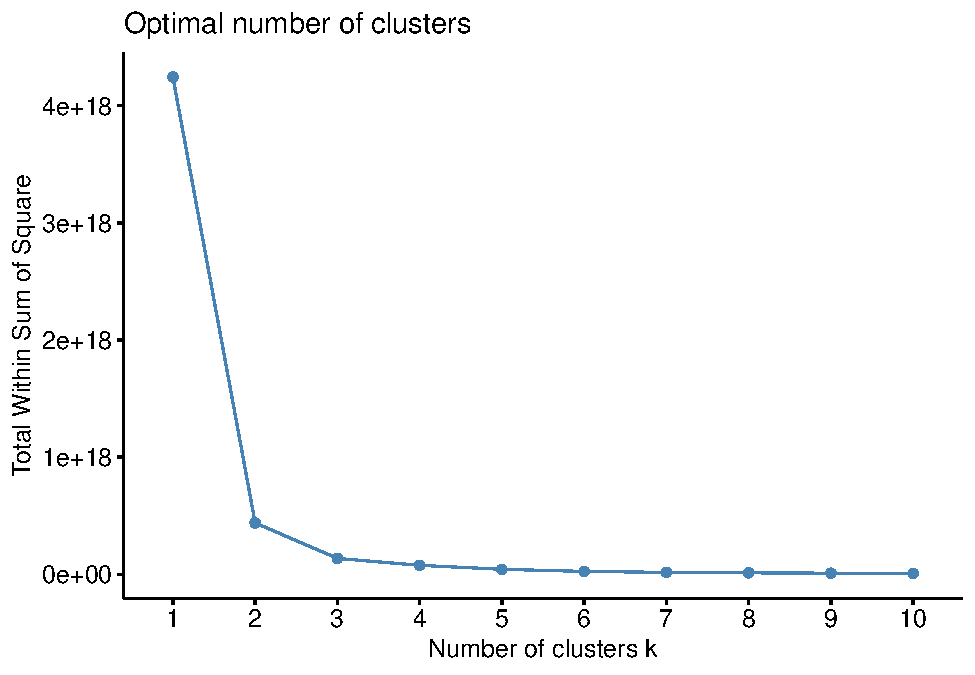
\includegraphics{Assignment1_files/figure-latex/pressure-1.pdf}

The dataset is very small and this results in Clara performing worse than PAM.

This code was optimised for reading

\hypertarget{refs}{}
\leavevmode\hypertarget{ref-WorldInData}{}%
European Center for Disease Prevention and Control. 2020. \emph{Coronavirus Source Data}. \url{https://ourworldindata.org/coronavirus-source-data}.

\end{document}
